\documentclass[aspectratio=169,11pt]{beamer}
\usepackage[T1]{fontenc}
\usepackage[utf8]{inputenc}
\usepackage{lmodern,amsmath,amssymb,graphicx,tikz}
\usetikzlibrary{arrows.meta,calc}
\usetheme{default}
\usefonttheme{serif}
\setbeamercolor{normal text}{fg=black,bg=white}
\setbeamercolor{structure}{fg=black}
\setbeamercolor{frametitle}{fg=black}
\setbeamercolor{title}{fg=black}
\setbeamertemplate{navigation symbols}{}
\setbeamertemplate{footline}[frame number]
\setbeamertemplate{itemize items}[circle]
\setbeamersize{text margin left=8mm,text margin right=8mm}
\setlength{\parskip}{5pt}
\newcommand{\cO}{\mathcal O}
\newcommand{\cI}{\mathcal I}
\newcommand{\cA}{\mathcal A}
\newcommand{\db}{\bar\partial}
\newcommand{\C}{\mathbb C}
\newcommand{\Pj}{\mathbb P}
\newcommand{\norm}[1]{\lVert#1\rVert}
\newcommand{\src}[1]{\par\vfill{\scriptsize #1\par}}
\author{Daniel Gonz\'alez Casanova Azuela}

\title{From curvature to Nadel vanishing}
\subtitle{Lecture 23 --- draft}
\date{Hodge theory}
\begin{document}
\begin{frame}\titlepage\end{frame}
\begin{frame}{What we want from vanishing}
Let \(A\) be a line bundle and \(x\in X\).
\[
0\longrightarrow A\otimes\mathfrak m_x
\longrightarrow A\longrightarrow A_x\longrightarrow0.
\]
The cohomology sequence contains
\[
H^0(X,A)\longrightarrow A_x
\longrightarrow H^1(X,A\otimes\mathfrak m_x).
\]
If the last group vanishes, we can prescribe a section's value at \(x\).
\par Here \(A_x\) denotes the fibre, regarded as a skyscraper sheaf in the sequence.
\end{frame}

\begin{frame}{The theorem we need}
Let \((X,\omega)\) be compact Kähler, \(\dim_{\C}X=n\).
Let \(B\) carry a singular Hermitian metric \(h\) with
\[
i\Theta_h\ge\varepsilon\omega,\qquad \varepsilon>0
\]
as currents. Nadel's theorem says
\[
\boxed{H^q(X,K_X\otimes B\otimes\cI_h)=0,\qquad q>0.}
\]
We must explain both the ideal \(\cI_h\) and the analytic estimate.
\end{frame}

\begin{frame}{Start with a norm on a line bundle}
Choose a local holomorphic frame \(e\) of \(B\).
Write
\[
|e|_h^2=e^{-2\varphi}.
\]
A section is \(s=fe\), so
\[
|s|_h^2=|f|^2e^{-2\varphi}.
\]
For a smooth metric, \(\varphi\) is smooth.
For a singular metric, we allow a locally integrable weight.
\end{frame}

\begin{frame}{From a fibre norm to an integral}
The metric on \(B\), together with \(\omega\), gives
\[
\norm{u}_h^2=\int_X |u|_{h,\omega}^2\,dV_\omega.
\]
For a holomorphic section \(fe\) on a coordinate ball, local integrability means
\[
\int_U |f|^2e^{-2\varphi}\,dV<\infty.
\]
A weight blowing up near a point can force \(f\) to vanish there.
\end{frame}

\begin{frame}{The multiplier ideal}
\[
\boxed{(\cI_h)_x=
\left\{f\in\cO_{X,x}:
|f|^2e^{-2\varphi}\text{ is integrable near }x\right\}.}
\]
It is an ideal: sums remain integrable, and holomorphic multipliers are locally bounded.
\medskip
\par The ideal consists of \emph{functions}.
The corresponding integrable holomorphic sections form \(B\otimes\cI_h\).
\end{frame}

\begin{frame}{Why this does not depend on the frame}
If \(e'=ge\), with \(g\) nowhere zero, then
\[
e^{-2\varphi'}=|g|^2e^{-2\varphi}.
\]
The factor \(|g|^2\) is bounded above and below on smaller neighbourhoods.
\[
|f|^2e^{-2\varphi'}\in L^1_{\mathrm{loc}}
\quad\Longleftrightarrow\quad
|f|^2e^{-2\varphi}\in L^1_{\mathrm{loc}}.
\]
The local ideals therefore glue.
\end{frame}

\begin{frame}{A weight that detects vanishing}
On \(\C^n\), put
\[
\varphi(z)=a\log|z|,
\qquad e^{-2\varphi}=|z|^{-2a}.
\]
Let \(k=\operatorname{ord}_0(f)\).
In polar coordinates, the relevant radial integral is
\[
\int_0^\delta r^{\,2k-2a+2n-1}\,dr.
\]
The leading homogeneous term of \(f\) gives this exponent.
\end{frame}

\begin{frame}{Where is the integrability threshold?}
\[
\int_0^\delta r^\beta\,dr<\infty
\quad\Longleftrightarrow\quad \beta>-1.
\]
Thus
\[
\boxed{|f|^2|z|^{-2a}\in L^1_{\mathrm{loc}}
\quad\Longleftrightarrow\quad k+n>a.}
\]
At equality the integral is \(\int dr/r\): it diverges.
\end{frame}

\begin{frame}{Picture: integrability switches on}
\begin{center}
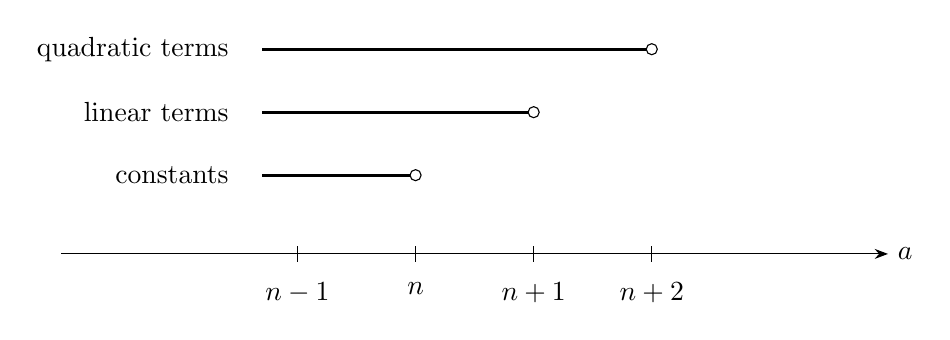
\begin{tikzpicture}[x=1.5cm,y=1cm]
\draw[-{Stealth}] (0,0)--(7,0) node[right] {\(a\)};
\foreach \x/\lab in {2/{n-1},3/{n},4/{n+1},5/{n+2}} {
 \draw (\x,.1)--(\x,-.1) node[below=4pt] {\(\lab\)};}
\node[anchor=east] at (1.5,1) {constants};
\draw[very thick] (1.7,1)--(3,1); \draw[fill=white] (3,1) circle (2pt);
\node[anchor=east] at (1.5,1.8) {linear terms};
\draw[very thick] (1.7,1.8)--(4,1.8); \draw[fill=white] (4,1.8) circle (2pt);
\node[anchor=east] at (1.5,2.6) {quadratic terms};
\draw[very thick] (1.7,2.6)--(5,2.6); \draw[fill=white] (5,2.6) circle (2pt);
\end{tikzpicture}
\end{center}
A term of degree \(k\) is allowed precisely when \(a<k+n\).
\[
a=n:\quad\cI_h=\mathfrak m_0,
\qquad
a=n+1:\quad\cI_h=\mathfrak m_0^2.
\]
\end{frame}

\begin{frame}{What does positive curvature mean here?}
In our convention,
\[
i\Theta_h=2i\partial\db\varphi.
\]
For a smooth weight this is a real \((1,1)\)-form:
\[
i\Theta_h=i\sum_{j,k}c_{j\bar k}\,dz_j\wedge d\bar z_k.
\]
Positivity means that the Hermitian matrix \((c_{j\bar k})\) is positive.
\par It is the curvature of \(B\), not sectional curvature of \(X\).
\end{frame}

\begin{frame}{Singular weights: positivity as a current}
Distributional differentiation still defines \(2i\partial\db\varphi\).
\[
i\Theta_h\ge\varepsilon\omega
\]
means \(i\Theta_h-\varepsilon\omega\) is a positive current.
\medskip
\par Locally, after subtracting a smooth potential for \(\varepsilon\omega\), the weight is plurisubharmonic.
\par This is where psh functions enter Nadel's theorem itself.
\end{frame}

\begin{frame}{Recall Bochner--Kodaira}
For a smooth Hermitian metric on \(B\),
\[
\Delta_{\db_B}=\Delta_{\partial_B}
+[i\Theta_B\wedge,\Lambda],
\qquad \Lambda=(\omega\wedge)^*.
\]
We use the identity from lecture 16 (Vanya).
\medskip
\par The useful part is a lower bound for the last operator on \((n,q)\)-forms.
\end{frame}

\begin{frame}{Diagonalize the curvature}
At a point, choose a unitary coframe such that
\[
\omega=i\sum_j dz_j\wedge d\bar z_j,
\qquad
i\Theta_B=i\sum_j\lambda_j\,dz_j\wedge d\bar z_j.
\]
Write
\[
u=\sum_{|J|=q}u_J\,dz_1\wedge\cdots\wedge dz_n\wedge d\bar z_J.
\]
On the \(J\)-term, \([i\Theta_B\wedge,\Lambda]\) acts by
\(\sum_{j\in J}\lambda_j\).
\end{frame}

\begin{frame}{The estimate we keep using}
If \(\lambda_j\ge\varepsilon\), then
\[
\left\langle[i\Theta_B\wedge,\Lambda]u,u\right\rangle
\ge q\varepsilon\norm{u}^2.
\]
Integrating Bochner--Kodaira gives
\[
\boxed{\norm{\db u}^2+\norm{\db^*u}^2
\ge q\varepsilon\norm{u}^2.}
\]
The omitted \(\partial_B\)-energy is nonnegative.
\end{frame}

\begin{frame}{Kodaira vanishing in three steps}
\[
H^q(X,K_X\otimes B)=0\qquad(q>0)
\]
when \(h\) is smooth and strictly positive.
\begin{enumerate}
\item Dolbeault identifies classes with \(B\)-valued \((n,q)\)-forms.
\item Hodge theory gives a harmonic representative \(u\).
\item The estimate gives \(0\ge q\varepsilon\norm{u}^2\), hence \(u=0\).
\end{enumerate}
This recalls Kodaira vanishing from lecture 16 (Vanya).
\end{frame}

\begin{frame}{What must change for Nadel?}
Our metric is singular, and our sheaf is now
\[
K_X\otimes B\otimes\cI_h.
\]
We need two replacements:
\begin{enumerate}
\item a Dolbeault resolution using locally \(L^2_h\) forms;
\item an \(L^2_h\) solution of \(\db u=f\).
\end{enumerate}
We cannot simply invoke the smooth compact Hodge theorem for this metric.
\end{frame}

\begin{frame}{Dolbeault, with an integrability condition}
\begin{columns}[c]
\column{.34\textwidth}
\centering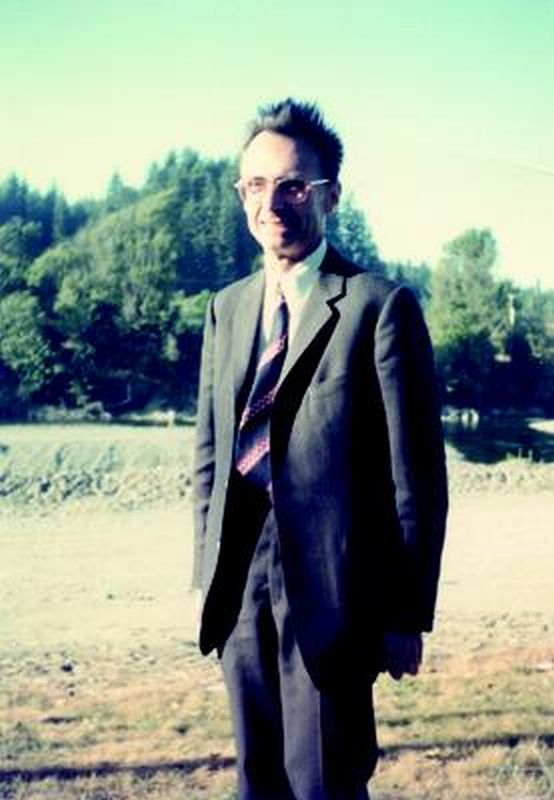
\includegraphics[height=4.7cm]{../assets/Pierre_Dolbeault.jpg}
\column{.62\textwidth}
The same architecture as our earlier Dolbeault proof:
\[
\text{local exactness}+\text{fine sheaves}
\]
computes sheaf cohomology by a global complex.
\medskip
\par We now put a weight into that complex.
\end{columns}
\src{Pierre Dolbeault. Portrait reused from the repository's \texttt{dbar-poincare} slides.}
\end{frame}

\begin{frame}{The sheaves of weighted forms}
Let \(\cA_h^{n,q}(U)\) consist of \(B\)-valued forms \(u\) such that
\[
u\in L^2_{\mathrm{loc}}(U,h),
\qquad
\db u\in L^2_{\mathrm{loc}}(U,h).
\]
The derivative is taken in the sense of distributions.
\medskip
\par No smoothness of \(u\) is required.
\par These are the maximal local domains of \(\db\).
\end{frame}

\begin{frame}{The kernel in degree zero}
A distributional solution of \(\db u=0\) in degree \((n,0)\) is holomorphic.
Locally it has the form
\[
u=f\,dz_1\wedge\cdots\wedge dz_n\otimes e.
\]
Its \(L^2_h\) condition is exactly
\[
|f|^2e^{-2\varphi}\in L^1_{\mathrm{loc}}.
\]
Therefore
\[
\ker(\db:\cA_h^{n,0}\to\cA_h^{n,1})
=K_X\otimes B\otimes\cI_h.
\]
\end{frame}

\begin{frame}{Local exactness: the analytic input}
\textbf{Weighted local \(\db\)-lemma.}
On a sufficiently small coordinate ball, a closed, locally \(L^2_h\)
\((n,q)\)-form \(f\), \(q>0\), has a locally \(L^2_h\) primitive:
\[
\db u=f.
\]
This is the weighted \(L^2\) version of the local lemma.
\medskip
\par Its proof uses the \(\db\) estimate with psh weights.
\end{frame}

\begin{frame}{Why local strict positivity is available}
On a small ball, replace \(\varphi\) by
\[
\widetilde\varphi=\varphi+C|z|^2.
\]
For large \(C\), the new curvature is strictly positive.
On a smaller ball,
\[
e^{-2C|z|^2}
\]
is bounded above and below by positive constants.
\par Thus the locally integrable forms and the multiplier ideal do not change.
\end{frame}

\begin{frame}{What approximation does locally}
Regularize a psh weight on smaller balls:
\[
\varphi_j\searrow\varphi,
\qquad e^{-2\varphi_j}\nearrow e^{-2\varphi}.
\]
Solve \(\db u_j=f\) for the smooth weights, with a uniform bound.
\medskip
\par Weak compactness gives a limit \(u\).
The distributional equation survives, and lower semicontinuity gives the weighted bound.
\par The uniform estimate is the essential ingredient.
\end{frame}

\begin{frame}{Why these sheaves are fine}
Multiply by a smooth function \(\chi\).
\[
\db(\chi u)=\db\chi\wedge u+\chi\,\db u.
\]
On relatively compact sets, \(\chi\) and its derivatives are bounded.
Both terms are locally \(L^2_h\).
\medskip
\par Smooth partitions of unity therefore act on \(\cA_h^{n,q}\).
These sheaves are fine.
\end{frame}

\begin{frame}{We have a fine resolution}
\[
0\longrightarrow K_X\otimes B\otimes\cI_h
\longrightarrow\cA_h^{n,0}
\xrightarrow{\db}\cA_h^{n,1}
\xrightarrow{\db}\cdots .
\]
Hence
\[
H^q(X,K_X\otimes B\otimes\cI_h)
=
\frac{\ker(\db:\Gamma\cA_h^{n,q}\to\Gamma\cA_h^{n,q+1})}
{\operatorname{im}(\db:\Gamma\cA_h^{n,q-1}\to\Gamma\cA_h^{n,q})}.
\]
On compact \(X\), local \(L^2_h\) integrability gives global \(L^2_h\) integrability.
\end{frame}

\begin{frame}{The remaining problem is one equation}
Take a class represented by \(f\):
\[
f\in L^2_h(X,\Lambda^{n,q}T^*X\otimes B),
\qquad \db f=0.
\]
To kill its cohomology class, we need
\[
\boxed{\db u=f,\qquad \norm{u}_h<\infty.}
\]
Existence without the weighted bound would not suffice.
\end{frame}

\begin{frame}{How an estimate produces a solution}
Temporarily use a smooth metric.
Set
\[
H_q=L^2(X,\Lambda^{n,q}T^*X\otimes B),\quad
T=\db:H_{q-1}\to H_q,\quad S=\db:H_q\to H_{q+1}.
\]
We know \(ST=0\), and
\[
\norm{T^*v}^2+\norm{Sv}^2\ge c\norm{v}^2,
\qquad c=q\varepsilon.
\]
The operators have their closed \(L^2\) domains.
\end{frame}

\begin{frame}{Restrict the target to closed forms}
Let \(Z=\ker S\), and regard \(T\) as
\[
T_0:\operatorname{Dom}T\subset H_{q-1}\longrightarrow Z.
\]
For \(v\in\operatorname{Dom}T_0^*\),
\[
\norm{v}\le c^{-1/2}\norm{T_0^*v}.
\]
Here \(T_0^*\) is \(T^*\) restricted to \(Z\).
\par We now solve against a given \(f\in Z\).
\end{frame}

\begin{frame}{Define the functional}
On \(\operatorname{im}T_0^*\), define
\[
\ell(T_0^*v)=\langle v,f\rangle.
\]
The estimate makes this well defined and gives
\[
|\ell(T_0^*v)|
\le \norm{v}\norm{f}
\le c^{-1/2}\norm{f}\norm{T_0^*v}.
\]
So \(\ell\) is a bounded functional.
\end{frame}

\begin{frame}{Hahn--Banach, then Riesz}
Extend \(\ell\) to \(H_{q-1}\), with the same norm.
Riesz gives a vector \(u\) such that
\[
\langle T_0^*v,u\rangle=\langle v,f\rangle,
\qquad \norm{u}\le c^{-1/2}\norm{f}.
\]
This is the adjoint definition of
\[
T_0u=f.
\]
Thus \(\db u=f\), and \(\norm{u}^2\le c^{-1}\norm{f}^2\).
\end{frame}

\begin{frame}{The singular-weight existence theorem}
\textbf{Analytic input.}
If \(i\Theta_h\ge\varepsilon\omega\) on compact Kähler \(X\), then for \(q>0\),
\[
\db f=0,\quad \norm{f}_h<\infty
\quad\Longrightarrow\quad
\db u=f,\qquad
\boxed{\norm{u}_h^2\le\frac{1}{q\varepsilon}\norm{f}_h^2.}
\]
This is the singular-weight extension of the preceding argument.
\par The theorem includes the required operator-domain and approximation statements.
\end{frame}

\begin{frame}{What the analytic extension must justify}
\begin{enumerate}
\setlength{\itemsep}{10pt}
\item Regularize the weights on suitable local or exhausted domains.
\item Apply the smooth estimate with controlled curvature errors and boundary terms.
\item Pass to weak limits while keeping the \(L^2_h\) bound.
\end{enumerate}
\medskip
This is a substantial analytic lemma.
A singular metric need not admit a global smooth approximation preserving strict positivity.
\end{frame}

\begin{frame}{Now prove Nadel}
\begin{enumerate}
\setlength{\itemsep}{9pt}
\item Represent a class by a global closed \(L^2_h\) form \(f\).
\item Apply singular-weight existence to obtain \(u\in L^2_h\) with \(\db u=f\).
\item Then \(u\) lies in the domain of the weighted complex.
\item Our class is exact, hence zero.
\end{enumerate}
\[
\boxed{H^q(X,K_X\otimes B\otimes\cI_h)=0\quad(q>0).}
\]
\end{frame}

\begin{frame}{Where did the canonical bundle come from?}
A \(B\)-valued \((n,q)\)-form is the same as a
\(K_X\otimes B\)-valued \((0,q)\)-form.
\[
\text{positive curvature on }B
\quad\Longrightarrow\quad
H^q(X,K_X\otimes B\otimes\cI_h)=0.
\]
To obtain a statement about a chosen line bundle \(A\), put
\[
\boxed{B=A\otimes K_X^{-1}.}
\]
\end{frame}

\begin{frame}{Return to the point (x)}
Suppose \(B=A\otimes K_X^{-1}\) has an admissible metric with
\[
\cI_h=\mathfrak m_x.
\]
Nadel gives \(H^1(X,A\otimes\mathfrak m_x)=0\).
Hence
\[
H^0(X,A)\twoheadrightarrow A_x.
\]
A prescribed nonzero fibre value lifts to a global holomorphic section.
\end{frame}

\begin{frame}{What Nadel has not constructed for us}
We still have to build a metric satisfying \emph{both}
\[
i\Theta_h\ge\varepsilon\omega
\qquad\text{and}\qquad
\cI_h=\mathfrak m_x.
\]
The local model \(n\log|z-x|\) gives the correct ideal.
\medskip
\par Gluing it into a global metric may introduce negative curvature.
Positive tensor powers will pay for that loss.
\end{frame}

\begin{frame}{Why this ideal appeared historically}
Nadel's 1990 paper studies the existence of Kähler--Einstein metrics.
\medskip
\par When an analytic estimate in that problem fails, a multiplier ideal records the concentration of the weights.
\medskip
\par Here we deliberately choose the singularities so that the ideal records the vanishing we want from sections.
\src{A. M. Nadel, \emph{Annals of Mathematics} 132 (1990), 549--596. DOI: 10.2307/1971429.}
\end{frame}

\begin{frame}{Two uses of the same theorem}
\begin{center}
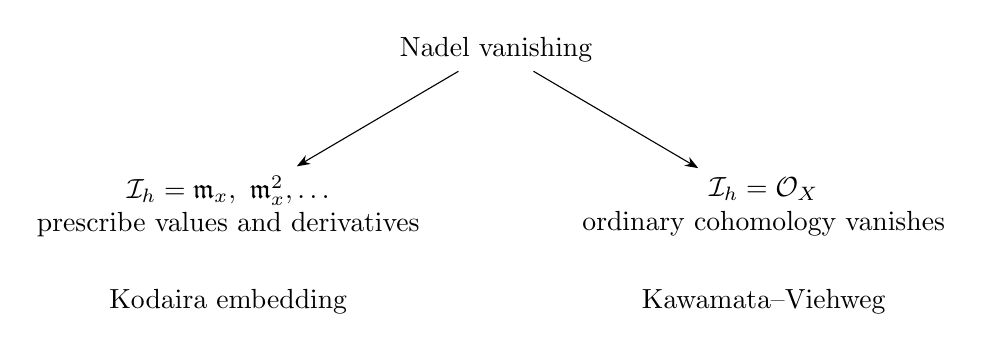
\begin{tikzpicture}[every node/.style={align=center},>=Stealth]
\node (n) at (0,2) {Nadel vanishing};
\node (a) at (-3.4,0) {\(\cI_h=\mathfrak m_x,\ \mathfrak m_x^2,\ldots\)\\prescribe values and derivatives};
\node (b) at (3.4,0) {\(\cI_h=\cO_X\)\\ordinary cohomology vanishes};
\draw[->] (n)--(a); \draw[->] (n)--(b);
\node at (-3.4,-1.2) {Kodaira embedding};
\node at (3.4,-1.2) {Kawamata--Viehweg};
\end{tikzpicture}
\end{center}
\end{frame}

\begin{frame}{Checkpoint before the applications}
\begin{enumerate}
\setlength{\itemsep}{10pt}
\item Why is \(\cI_h\) an ideal of functions, rather than a space of global sections?
\item Why does the threshold \(a=n\) exclude constants?
\item Where did we use positivity?
\item Where did we use compactness?
\end{enumerate}
\end{frame}

\begin{frame}{Proof map to keep on the board}
\[
\text{curvature lower bound}
\ \Longrightarrow\
L^2\text{ estimate}
\ \Longrightarrow\
\db\text{ solvability}.
\]
\[
\text{weighted local lemma}
\ \Longrightarrow\
\text{fine resolution}
\ \Longrightarrow\
\text{cohomology computed by }L^2_h\text{ forms}.
\]
Together these give Nadel vanishing.
\end{frame}

\begin{frame}{Reading and preparation}
\small
M. Verbitsky, \emph{Kähler geometry}, 2025 source for lecture 23 (Daniel): the course route to Nadel vanishing.
\medskip
\par J.-P. Demailly, \emph{\(L^2\) vanishing theorems for positive line bundles and adjunction theory} (1994), arXiv:alg-geom/9410022: analytic details.
\medskip
\par A. M. Nadel, \emph{Multiplier ideal sheaves and Kähler--Einstein metrics of positive scalar curvature} (1990): original context.
\medskip
\par The accompanying notes distinguish proofs given here from analytic inputs.
\end{frame}
\end{document}
